\section{How far apart were the planes?\\ \small{(%Pathway: Any; 
Pre-requisite: None)}}

%\item
%\underline{\large\bf How far apart were the planes?}  \\[0.1cm]
\begin{minipage}{9.5cm}
A news story from a few years ago alleged that two planes nearly collided
in mid-air. Indeed, the photo shows the two planes, an Airbus A-300
and a Boeing 777, very close to each other. However, the air-traffic
authorities maintained that the two planes were never in close proximity.
One of the difficulties in assessing photographic information is that
it has no depth, and the overlapping objects may in fact be quite
far from each other.
\end{minipage}
\hspace{0.3cm}
\begin{minipage}{6.5cm}
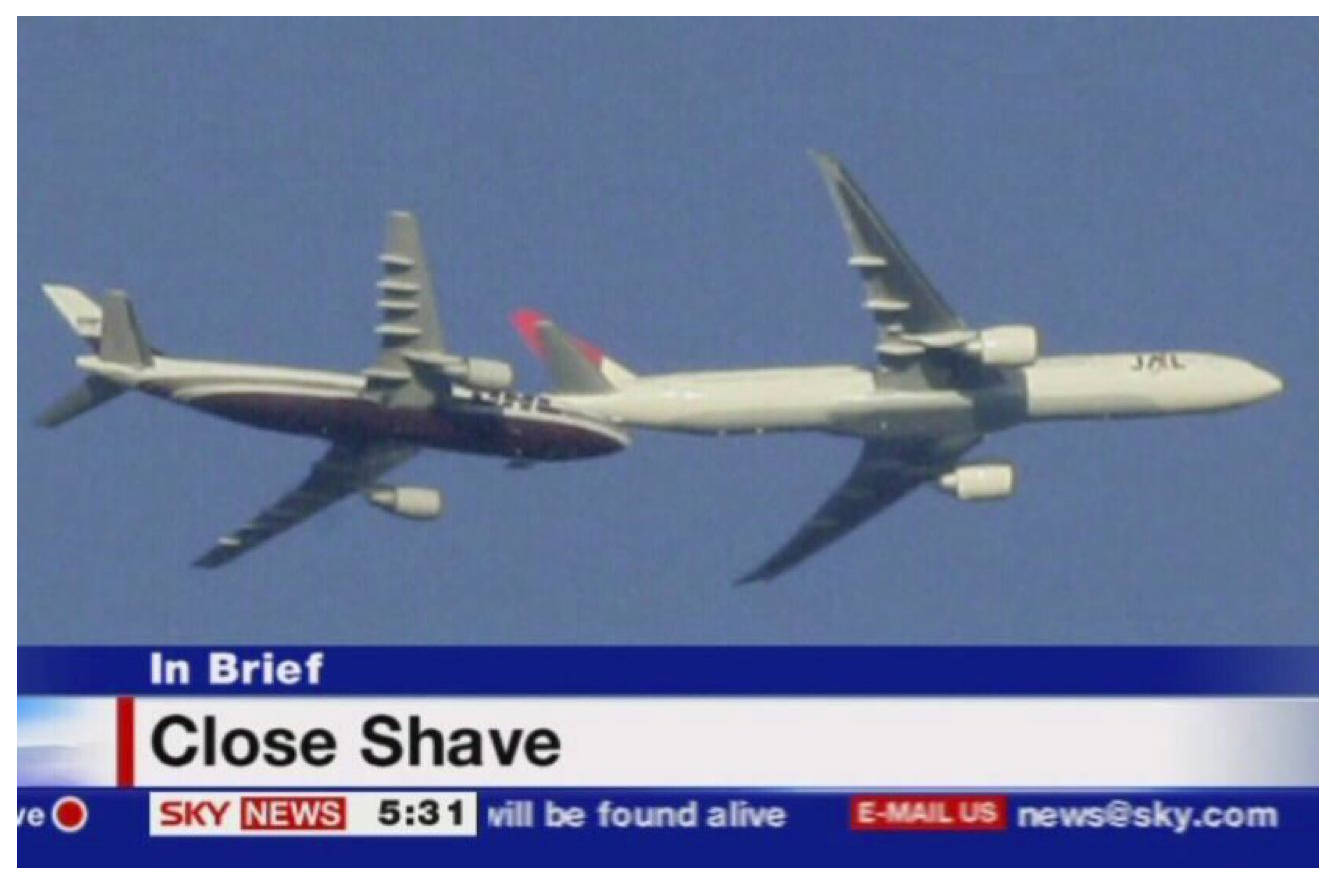
\includegraphics[angle=0,width=6.5cm]{projects/nearmiss1.eps}
\end{minipage}
%\begin{center}
%\includegraphics[angle=0,width=4cm]{2_planes.eps}
%\end{center}

\vspace{12pt}
The relative sizes of the planes in the photo can provide some information
about the {\em ratio} of the distances to the planes from the observer.
However, (i) the planes are not identical, and (ii) they are viewed at
different angles. Because of (ii) the length of the plane's
body in the photograph appears smaller than if the body is perpendicular to
the line of sight.\\[6pt]
Examine the top view of the plane (a) and its schematic kite-like
representation (b) in the diagram below. For common commercial aircraft, the
length HT and wingspan LR can be found easily. When the plane is seen at an
angle, as in diagram (c), the angle $\alpha $ between HT and LR is no
longer 90$^\circ $. The ratio of the visible wingspan, L$'$R$'$ to the visible
body length H$'$T$'$ is also different from what they are in (b).
\begin{center}
%\includegraphics[angle=-90,width=11cm]{plane_kite.pdf}
\includegraphics[angle=0,width=11cm]{projects/plane_kite.eps}
\end{center}
The task is to use the values of L$'$R$'$, H$'$T$'$ and $\alpha $
measured on the photograph, to determine what LR and HT  should be on
the photograph. One can then use this information (and the real aircaft
dimensions) to estimate how far apart the aircraft were, assuming that we
know the distance to one of them (e.g., 2 km, as the photo was taken with a
tele lens).
